\chapter{图片}


设置了图片caption与图片之间的距离;
\begin{lstlisting}
    \RequirePackage[labelfont={bf,color=structurecolor}]{caption} 
    \captionsetup[table]{skip=6pt} %表格
    \captionsetup[figure]{skip=6pt} %图片
\end{lstlisting}

\section{一行两张图}
设置一行两张图
\begin{figure}[htbp]
    \centering
    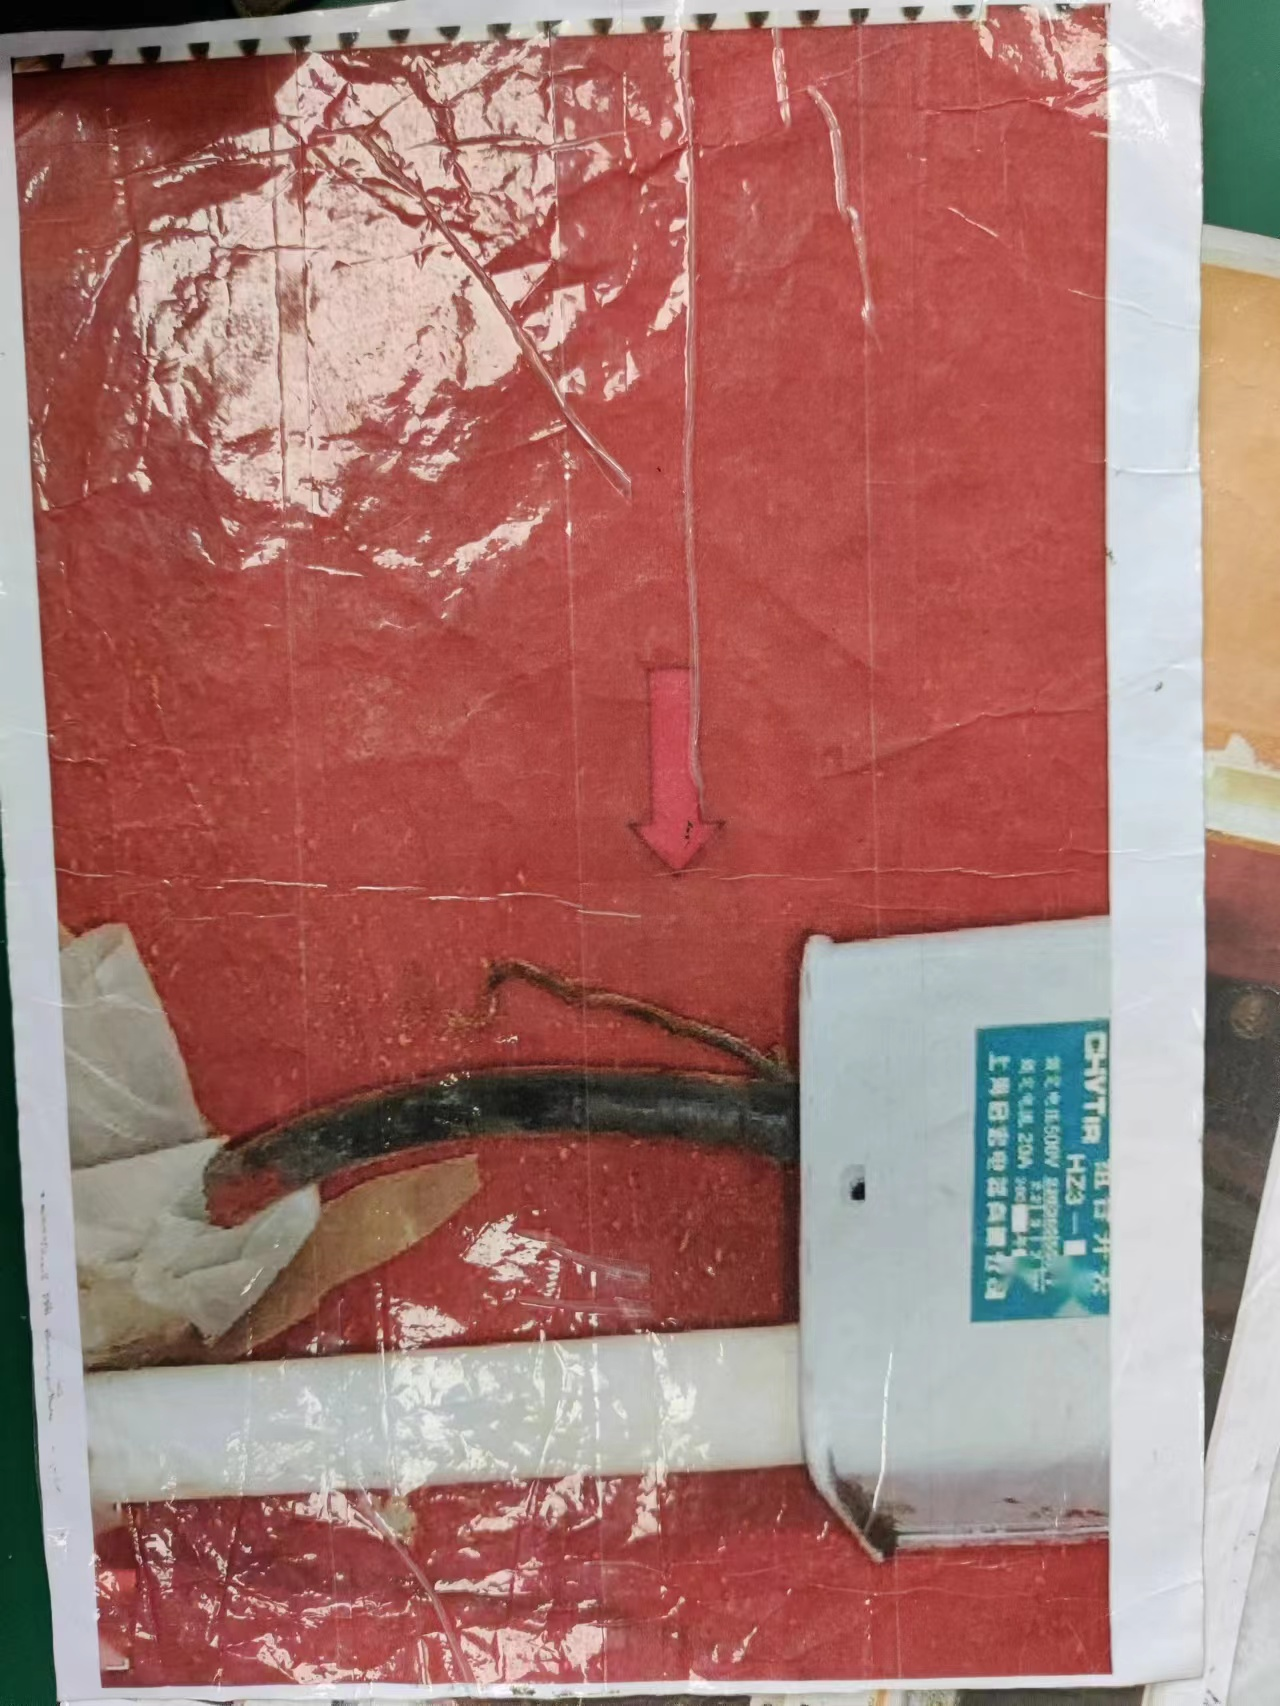
\includegraphics[width = 0.35\textwidth]{1}
    % \hfill
    \hspace*{1cm}
    % 
\includegraphics[width = 0.35\textwidth,trim = 500 200 300 400,clip,angle=0]{cover16}
    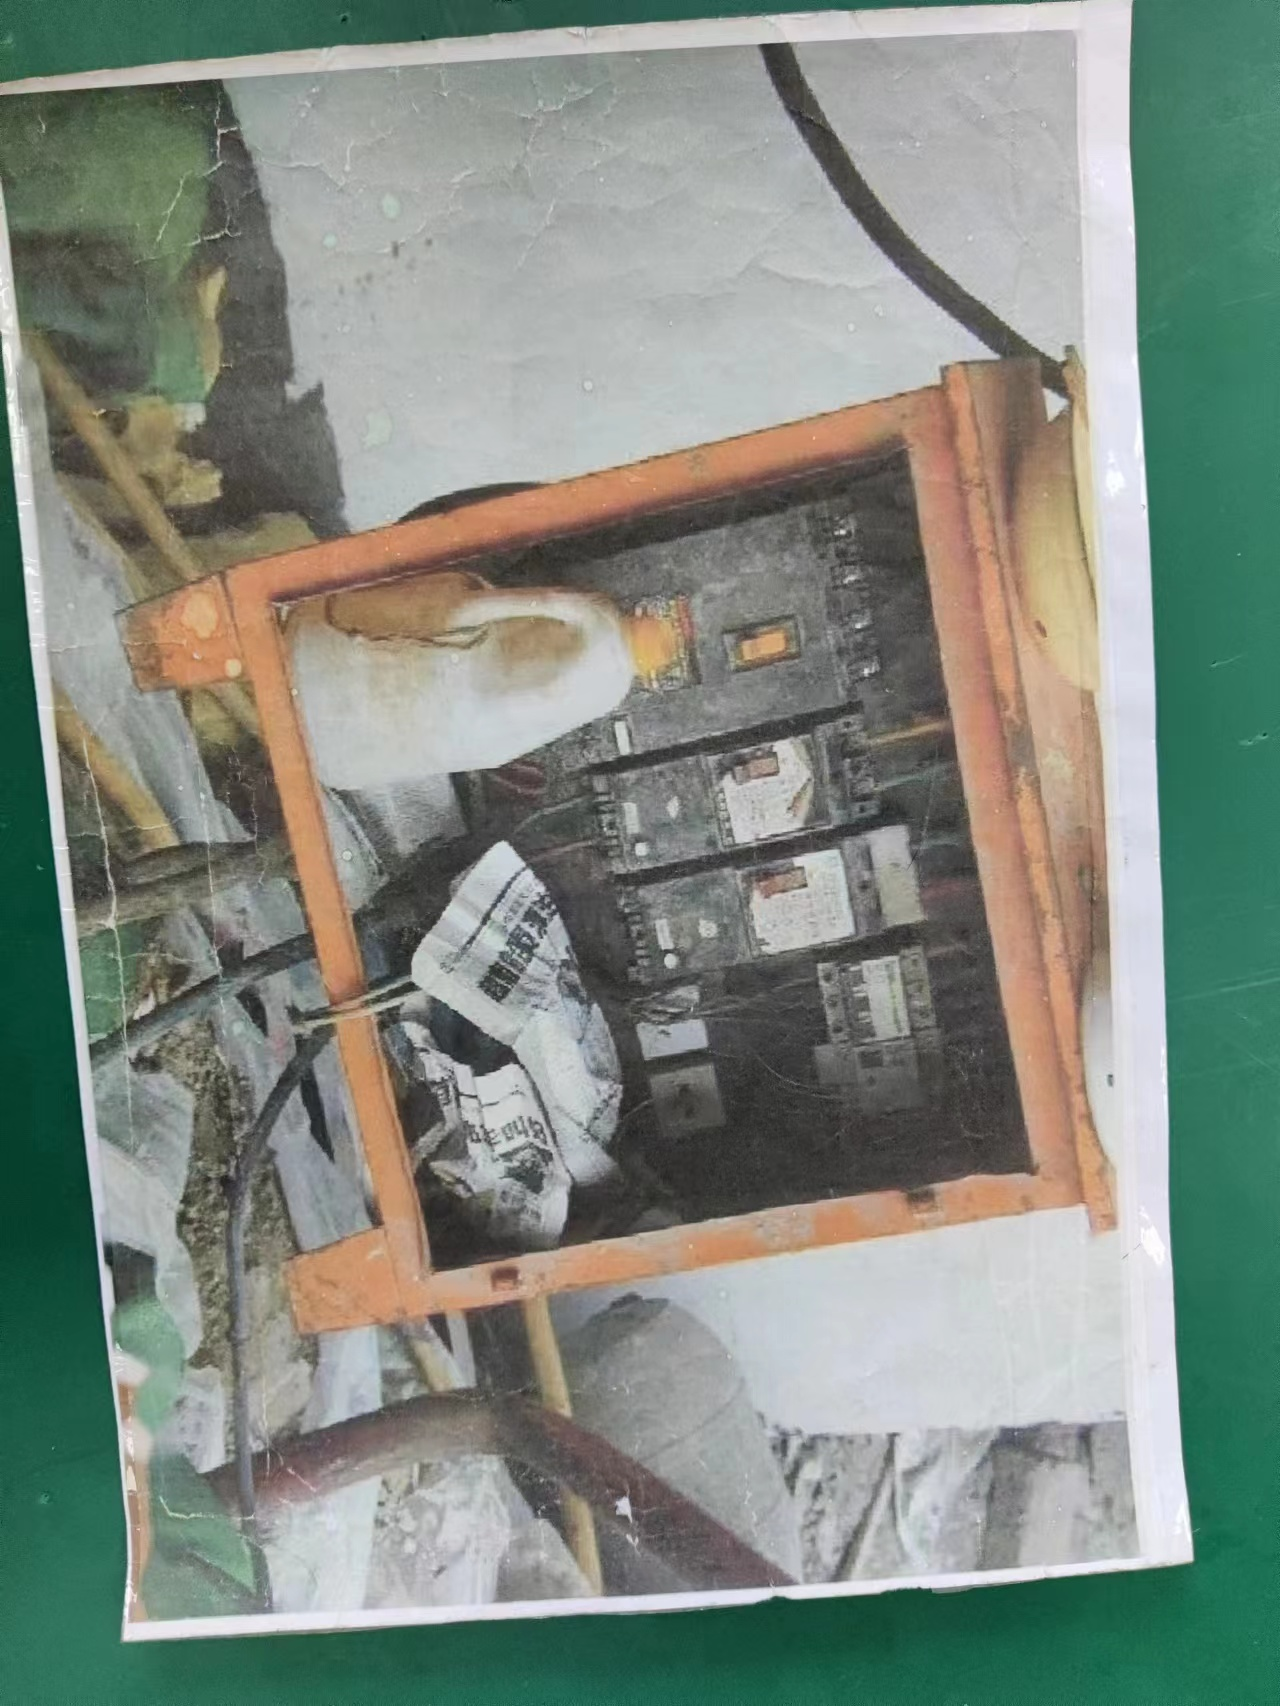
\includegraphics[width = 0.35\textwidth,angle=0]{3}
    \caption{有图有真相}
    \label{fig:myphoto}
\end{figure}


\section{一行两张图小标题}


\begin{figure}[!htbp]
    \centering
    \begin{minipage}[t]{0.45\textwidth}
        \centering
        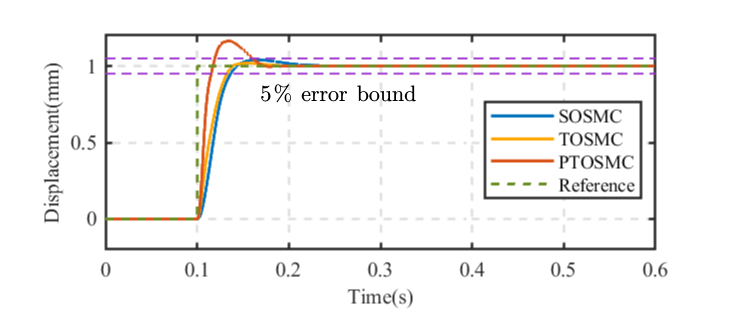
\includegraphics[width=\textwidth]{5-1} % 替换为你的图片文件名
        \caption{图像 1}
        \label{fig1a}
    \end{minipage}
    \begin{minipage}[t]{0.45\textwidth}
        \centering
        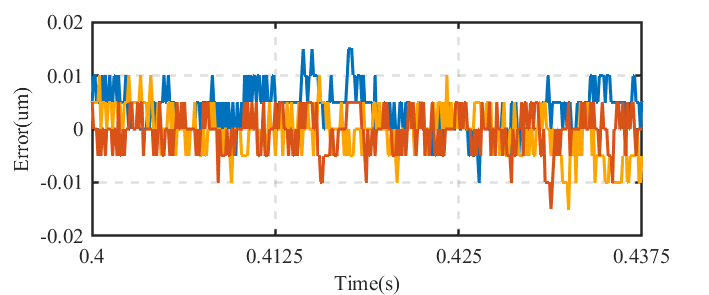
\includegraphics[width=\textwidth]{5-2} % 替换为你的图片文件名
        \caption{图像 2}
        \label{fig1b}
    \end{minipage}
    \caption{两个图像的并排显示}
    \label{fig1}
\end{figure}



\begin{figure}[!htbp]
    \centering
    \begin{subfigure}[b]{0.45\textwidth}
        \centering
        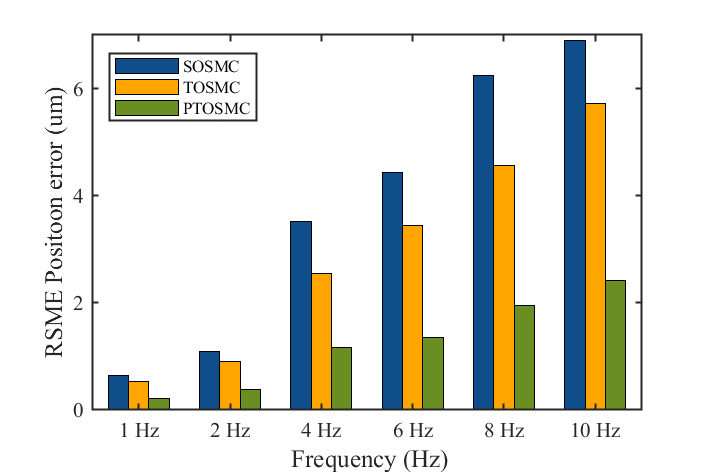
\includegraphics[width=\textwidth]{10} % 替换为你的图片文件名
        \caption{图像 1}
        \label{fig:sub1}
    \end{subfigure}
    \hspace*{1cm}
    \begin{subfigure}[b]{0.45\textwidth}
        \centering
        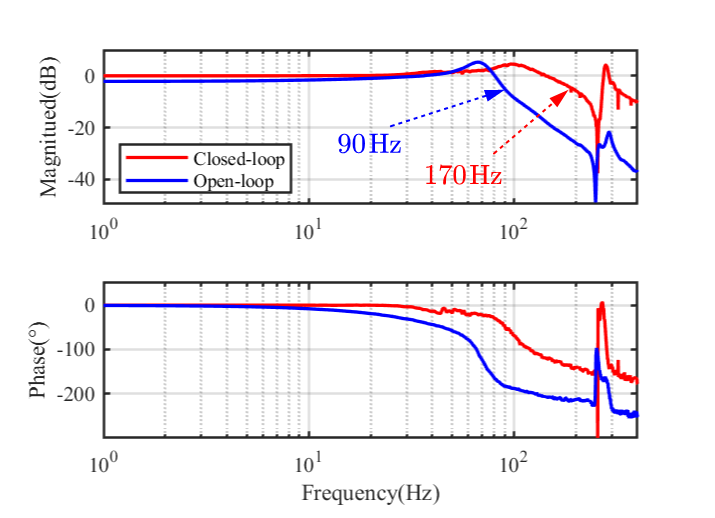
\includegraphics[width=\textwidth]{11} % 替换为你的图片文件名
        \caption{图像 2}
        \label{fig:sub2}
    \end{subfigure}
    \caption{两个图像的并排显示}
    \label{fig:main}
\end{figure}